\documentclass{standalone}
\usepackage{amsmath}
\usepackage{amssymb}
\usepackage{tikz}
\usetikzlibrary{positioning,arrows.meta,decorations.pathreplacing}
\begin{document}
	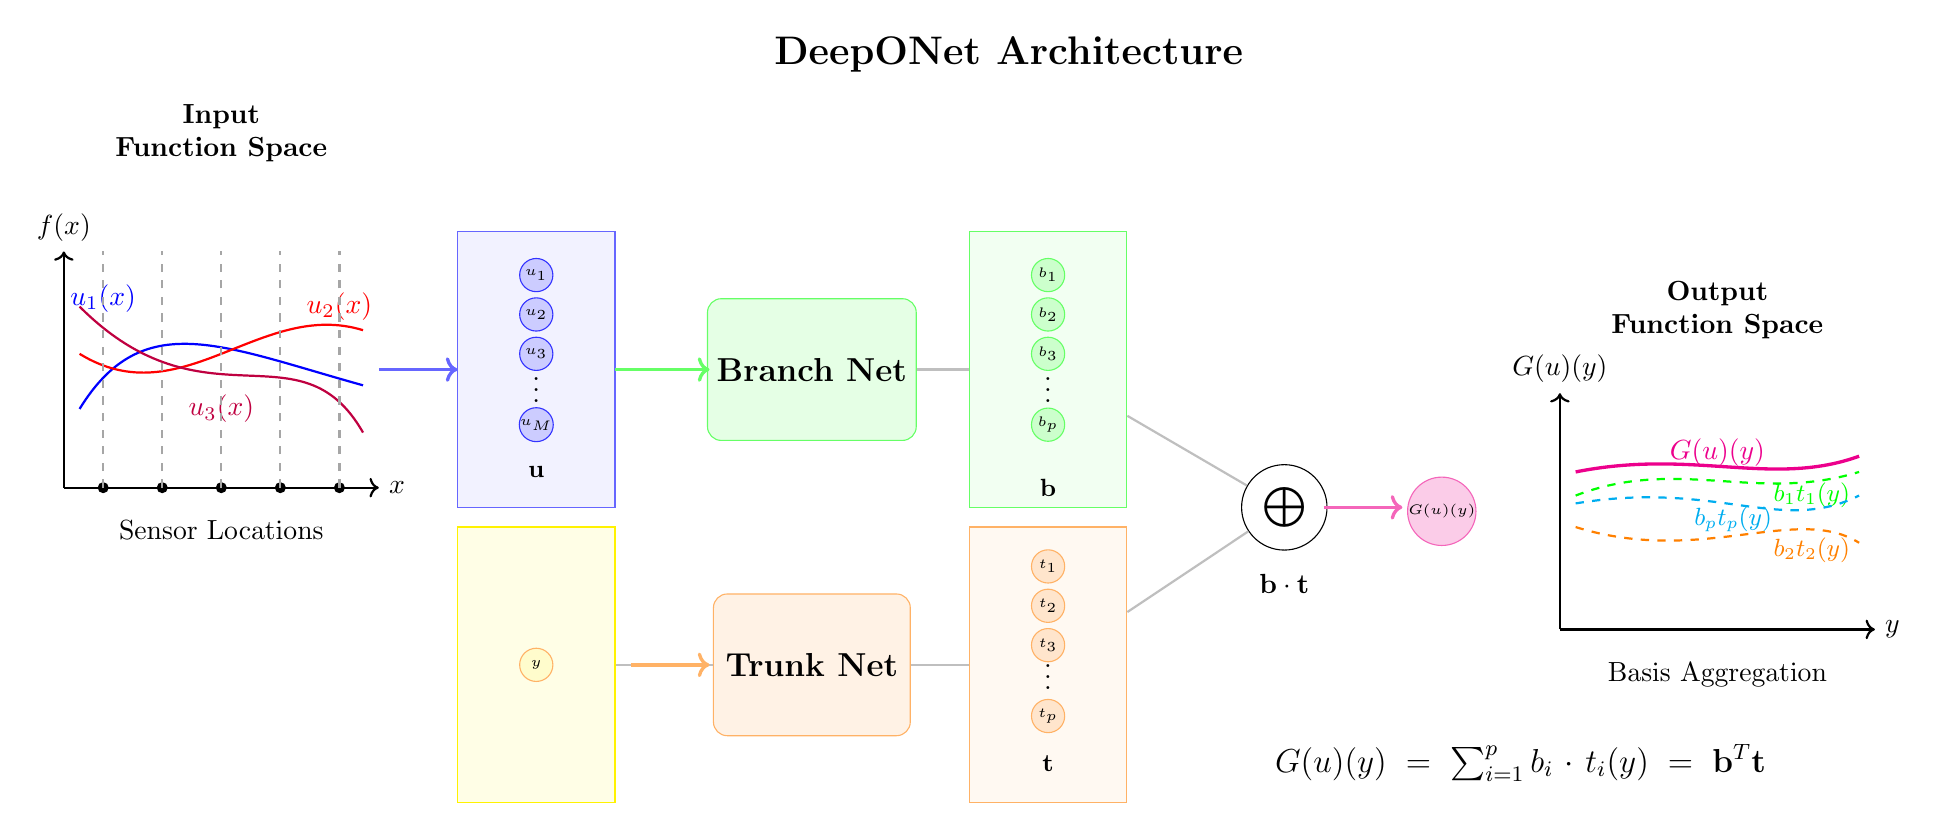
\begin{tikzpicture}[
		% Define styles for nodes and connections
		small_neuron/.style={circle, draw, minimum size=12pt, inner sep=0pt, font=\tiny},
		input_neuron/.style={small_neuron, fill=blue!20, draw=blue!80},
		branch_neuron/.style={small_neuron, fill=green!20, draw=green!60},
		trunk_neuron/.style={small_neuron, fill=orange!20, draw=orange!60},
		trunk_input_neuron/.style={small_neuron, fill=yellow!20, draw=orange!60},
		output_neuron/.style={small_neuron, fill=magenta!20, draw=magenta!60},
		vector_box/.style={rectangle, draw, minimum width=2cm, minimum height=3.5cm, fill=blue!5, draw=blue!60},
		branch_vector/.style={rectangle, draw, minimum width=2cm, minimum height=3.5cm, fill=green!5, draw=green!60},
		trunk_input_vector/.style={rectangle, draw, minimum width=2cm, minimum height=3.5cm, fill=yellow!10, draw=yellow!100},
		trunk_vector/.style={rectangle, draw, minimum width=2cm, minimum height=3.5cm, fill=orange!5, draw=orange!60},
		output_vector/.style={rectangle, draw, minimum width=2cm, minimum height=2.5cm, fill=magenta!5, draw=magenta!60},
		net/.style={rectangle, draw, rounded corners=5pt, minimum width=2.5cm, minimum height=1.8cm, text centered, font=\large\bfseries},
		branch_net/.style={net, fill=green!10, draw=green!60},
		trunk_net/.style={net, fill=orange!10, draw=orange!60},
		conn/.style={gray!50, line width=0.8pt},
		sensor/.style={circle, fill=black, inner sep=1pt, minimum size=4pt},
		func/.style={thick, smooth},
		dashed_line/.style={dashed, thick, gray!70},
		axis/.style={thick, ->}
		]
		
		% Input function space
		\node[text width=3cm, align=center, font=\bfseries] at (-2, 5) {Input\\ Function Space};
		
		% Input space axes
		\begin{scope}[shift={(-2, 2)}]
			% Axes
			\draw[axis] (-2, -1.5) -- (2, -1.5) node[right] {$x$};
			\draw[axis] (-2, -1.5) -- (-2, 1.5) node[above] {$f(x)$};
			
			% Bounding box for function space
			% \draw[thick, blue!60] (-2.2, -1.7) rectangle (2.2, 1.7);
			
			% Three input functions (cubic derivatives)
			\draw[func, blue, thick] (-1.8, -0.5) .. controls (-1, 0.8) and (0, 0.3) .. (1.8, -0.2);
			\node[blue] at (-1.5, 0.9) {$u_1(x)$};
			
			\draw[func, red, thick] (-1.8, 0.2) .. controls (-0.5, -0.6) and (0.5, 0.9) .. (1.8, 0.5);
			\node[red] at (1.5, 0.8) {$u_2(x)$};
			
			\draw[func, purple, thick] (-1.8, 0.8) .. controls (-0.2, -0.8) and (1, 0.6) .. (1.8, -0.8);
			\node[purple] at (0, -0.5) {$u_3(x)$};
			
			% Fixed sensor locations
			\foreach \x in {-1.5, -0.75, 0, 0.75, 1.5} {
				\node[sensor] at (\x, -1.5) {};
				\draw[dashed_line] (\x, -1.5) -- (\x, 1.5);
			}
			
			\node[below] at (0, -1.8) {Sensor Locations};
		\end{scope}
		
		% Input vector box with spacing
		\node[vector_box] (input_vec) at (2, 2) {};
		\node[input_neuron] (u1) at (2, 3.2) {$u_1$};
		\node[input_neuron] (u2) at (2, 2.7) {$u_2$};
		\node[input_neuron] (u3) at (2, 2.2) {$u_3$};
		\node[text centered] at (2, 1.85) {$\vdots$};
		\node[input_neuron] (uM) at (2, 1.3) {$u_M$};
		\node[text width=1.8cm, align=center, font=\small] at (2, 0.7) {$\mathbf{u}$};
		
		% Branch network with spacing
		\node[branch_net] (branch) at (5.5, 2) {Branch Net};
		
		% Branch vector box with spacing
		\node[branch_vector] (branch_vec) at (8.5, 2) {};
		\node[branch_neuron] (b1) at (8.5, 3.2) {$b_1$};
		\node[branch_neuron] (b2) at (8.5, 2.7) {$b_2$};
		\node[branch_neuron] (b3) at (8.5, 2.2) {$b_3$};
		\node[text centered] at (8.5, 1.85) {$\vdots$};
		\node[branch_neuron] (bp) at (8.5, 1.3) {$b_p$};
		\node[text width=1.8cm, align=center, font=\small] at (8.5, 0.5) {$\mathbf{b}$};
		
		% Query location input with spacing
		\node[trunk_input_vector] (query_vec) at (2, -1.75) {};
		\node[trunk_input_neuron] (y) at (2, -1.75) {$y$};
		
		% Trunk network with spacing
		\node[trunk_net] (trunk) at (5.5, -1.75) {Trunk Net};
		
		% Trunk vector box with spacing
		\node[trunk_vector] (trunk_vec) at (8.5, -1.75) {};
		\node[trunk_neuron] (t1) at (8.5, -0.5) {$t_1$};
		\node[trunk_neuron] (t2) at (8.5, -1.0) {$t_2$};
		\node[trunk_neuron] (t3) at (8.5, -1.5) {$t_3$};
		\node[text centered] at (8.5, -1.8) {$\vdots$};
		\node[trunk_neuron] (tp) at (8.5, -2.4) {$t_p$};
		\node[text width=1.8cm, align=center, font=\small] at (8.5, -3) {$\mathbf{t}$};
		
		% Dot product operation with spacing
		\node[circle, draw, minimum size=25pt, font=\Large] (dot) at (11.5, 0.25) {$\bigoplus$};
		\node[below=5pt of dot] {$\mathbf{b} \cdot \mathbf{t}$};
		
		% Output vector with spacing
		% \node[output_vector] (output_vec) at (14, 0.25) {};
		\node[output_neuron] (output) at (13.5, 0.2) {$G(u)(y)$};
		
		% Output function space with more spacing
		\node[text width=3cm, align=center, font=\bfseries] at (17, 2.75) {Output \\Function Space};
		
		\begin{scope}[shift={(17, 0.2)}]
			% Axes
			\draw[axis] (-2, -1.5) -- (2, -1.5) node[right] {$y$};
			\draw[axis] (-2, -1.5) -- (-2, 1.5) node[above] {$G(u)(y)$};
			
			% Bounding box for output function space
			% \draw[thick, magenta!60] (-2.2, -1.7) rectangle (2.2, 1.7);
			
			% Three basis functions
			\draw[func, green, thick, dashed] (-1.8, 0.2) .. controls (-0.5, 0.7) and (0.5, 0.1) .. (1.8, 0.5);
			\node[green] at (1.2, 0.2) {\small $b_1 t_1(y)$};
			
			\draw[func, orange, thick, dashed] (-1.8, -0.2) .. controls (-0.2, -0.7) and (1, 0.1) .. (1.8, -0.4);
			\node[orange] at (1.2, -0.5) {\small $b_2 t_2(y)$};
			
			\draw[func, cyan, thick, dashed] (-1.8, 0.1) .. controls (0, 0.4) and (0.8, -0.3) .. (1.8, 0.2);
			\node[cyan] at (0.2, -0.1) {\small $b_p t_p(y)$};
			
			% Sum of basis functions (final output)
			\draw[func, magenta, very thick] (-1.8, 0.5) .. controls (-0.3, 0.8) and (0.7, 0.3) .. (1.8, 0.7);
			\node[magenta, font=\bfseries] at (0, 0.75) {$G(u)(y)$};
			
			
			\node[below] at (0, -1.8) {Basis Aggregation};
		\end{scope}
		
		% Connections with proper spacing
		\draw[conn, thick] (input_vec) -- (branch);
		\draw[conn, thick] (branch) -- (branch_vec);
		\draw[conn, thick] (query_vec) -- (trunk);
		\draw[conn, thick] (trunk) -- (trunk_vec);
		\draw[conn, thick] (branch_vec) -- (dot);
		\draw[conn, thick] (trunk_vec) -- (dot);
		
		% Mathematical expression
		\node[text width=8cm, align=center, font=\large] at (14.5, -3.0) {
			$G(u)(y) = \sum_{i=1}^{p} b_i \cdot t_i(y) = \mathbf{b}^T \mathbf{t}$
		};
		
		% Title
		\node[font=\Large\bfseries] at (8, 6) {DeepONet Architecture};
		
		% Arrow showing data flow with proper spacing
		\draw[->, very thick, blue!60] (-0, 2) -- (1., 2);
		\draw[->, very thick, green!60] (3, 2) -- (4.2, 2);
		\draw[->, very thick, orange!60] (3.2, -1.75) -- (4.2, -1.75);
		\draw[->, very thick, magenta!60] (12., 0.25) -- (13, 0.25);
		
	\end{tikzpicture}
\end{document}